\documentclass[oneside,10pt]{article}
\usepackage[T1]{fontenc}
\usepackage[spanish,mexico]{babel}
\usepackage[papersize={148mm, 199.5mm}, top=7mm, bottom=13mm, left=13mm, right=13mm]{geometry}
\usepackage[utf8x]{inputenc}
\usepackage{amsthm}
\usepackage{amssymb}
\usepackage{amsmath}
\usepackage{blindtext}
\usepackage{graphicx}

\begin{document}
\author{Barragán Jim\'enez Jonathan}
\date{14 junio 2017\\ Facultad de Ciencias UNAM}
\title{Cubo Gen\'etico }
\maketitle


\section{Introducción}

El cubo de Rubik o cubo m\'agico fue inventado  por el escultor y profesor de arquitectura h\'ungaro Erno Rubik en 1974. El cubo de Rubik original (existen muchas variaciones pero s\'olo nos centraremos en el 3x3x3) tiene 8 v\'ertices y doce aristas. El problema consiste en encontrar el m\'inimo n\'umero de movimientos que se necesitan para llegar de un estado no resuelto al resuelto, partiendo del supuesto que  \textsl{El n\'umero de dios es 20}\cite{god20},  es decir cualquier posici\'on del cubo de Rubik se puede resolver en 20 movimientos o menos. \\ 

Hoy en d\'ia ya se conoce mucho sobre como resolver el cubo m\'agico o el cubo de 3x3x3, pero no existe un algortimo que pueda resolver el cubo de Rubik en 20 movimientos, ya que aunque se pueda hacer, estos movimeintos ser\'an totalmente distintos para cada posici\'on y tomando encuenta que el cubo tiene un total de :  \[ \frac{8! \cdot 12! \cdot 3^{7} \cdot 2^{11} }{2} = 43,252,003,274,489,856,000 \] permutaciones utilizaremos el algoritmo gen\'etico para tratar este problema.\\

Un algoritmo gen\'etico es una metaheuristica inspirada por el proceso de selecci\'on natural que pertenece a la clase de algoritmos evolutivos. En este reporte se muestra una implementaci\'on del algorimo gen\'etico mostrando la codificaci\'on y los operadores (selecci\'on, cruza, mutaci\'on). 

\newpage

\section{Desarrollo}
\subsection{Cubo 3x3x3}
Lo primero que haremos ser\'a modelar un cubo 3x3x3 como una matriz de 6x9 (\ref{tabla:matriz}) en donde cada cuadrante (por ejemplo i<3 y j<3 donde 0<=i<=5 y 0<=j<=8) representa una cara del cubo, tambi\'en para no complicarnos los colores del cubo los denotaremos con n\'umeros, es decir para los seis colores que tiene el cubo se les asignar\'a un n\'umero  (\ref{tabla:numcol}) (\ref{fig:ejemplo}).
\\
\begin{table}[htbp]
\begin{center}
\begin{tabular}{|c||c|c|c|c|c|c|c|c|c|}
\hline
&\textsl{0}&\textsl{1}&\textsl{2}&\textsl{3}&\textsl{4}&\textsl{5}&\textsl{6}&\textsl{7}&\textsl{8} \\
\hline \hline
\textsl{0}&1&1&1&2&2&2&3&3&3 \\
\hline
\textsl{1}&1&1&1&2&2&2&3&3&3 \\
\hline
\textsl{2}&1&1&1&2&2&2&3&3&3 \\
\hline
\textsl{3}&4&4&4&5&5&5&6&6&6 \\
\hline
\textsl{4}&4&4&4&5&5&5&6&6&6 \\
\hline
\textsl{5}&4&4&4&5&5&5&6&6&6 \\
\hline
\end{tabular}
\caption{Matriz 6x9 que reprensenta un cubo resuelto.}
\label{tabla:matriz}
\end{center}
\end{table}

\begin{table}[htbp]
\begin{center}
\begin{tabular}{|l|l|l|l|l|l|}
\hline
AZUL & ROJO & BLANCO & AMARILLO & NARANJA & VERDE \\
\hline
1 & 2 & 3 & 4 & 5 & 6 \\
\hline
\end{tabular}
\caption{Representaci\'on de los colores en la matriz.}
\label{tabla:numcol}
\end{center}
\end{table}

\newpage

\begin{figure}
  \begin{center}
  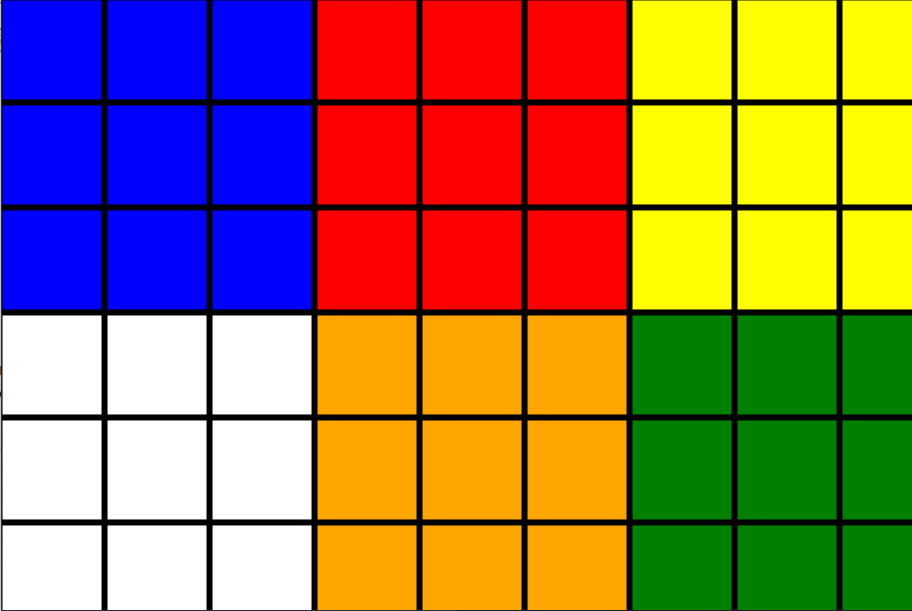
\includegraphics[width=0.7\textwidth]{migrafico}
  \caption{Representaci\'on ilustrada de la matriz}
  \label{fig:ejemplo}
  \end{center}
\end{figure}

\subsection{Genotipo y Fenotipo}
Para poder modelar a un individuo en el algoritmo gen\'etico necesitamos definir tanto su fenotipo y genotipo.
El Genotipo en Biolog\'ia , se refiere a la informaci\'on gen\'etica que posee un organismo y el Fenotipo en Biolog\'ia la realizaci\'on visible del genotipo en un determinado ambiente. En el algoritmo gen\'etico, el genotipo sera una forma de codificar la soluci\'on de un determinado problema para que sea mas f\'acil operar y el fenotipo es una representaci\'on de la soluci\'on que sea simple de entender por lo tanto un individuo sera representado por su genotipo y por su fenotipo.\\

\begin{figure}
  \begin{center}
  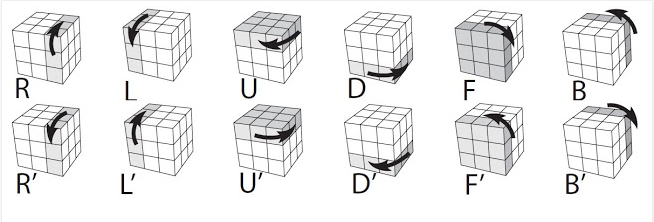
\includegraphics[width=0.7\textwidth]{notacion}
  \caption{Notaci\'on de un cubo 3x3x3 }
  \label{fig:move}
  \end{center}
\end{figure}

En nuestro problema un soluci\'on ser\'a representada como un arreglo de movimientos consecutivos de tama\~no menor o igual a 20. Para representar los movimientos ocuparemos la notaci\'on estandar en ingles de cubo 3x3x3 (\ref{fig:move}), entonces, un individuo en nuestra implimentaci\'on del algoritmo gen\'etico ser\'a representado(\ref{tabla:individuo}), (sin tomar encuenta los movientos dobles o medios ya que son facilmente realizables con movimientos simples), por su fenotipo que ser\'a el arreglo de caracteres con los movimentos y el genotipo ser\'a un arreglo de n\'umeros donde para cada movimiento le corresponde un n\'umero. Cabe mencionar que en una poblaci\'on puede existir individuos de diferentes tama\~nos.

\begin{table}[htbp]
\begin{center}
\begin{tabular}{|l|c|c|c|c|c|c|}
\hline
Fenotipo & R & B & F' & L & L'& D\\
\hline
Genotipo & 1 & 11 & 10 & 3 & 4 & 7\\
\hline
\end{tabular}
\caption{Representaci\'on de un Indivduo.}
\label{tabla:individuo}
\end{center}
\end{table}

\subsection{Funci\'on de aptitud (fitness)}
La funci\'on de aptitud(fitness) evalua al individuo para saber que tan apto es, es decir, que tan cercano est\'a de una soluci\'on \'optima, la funci\'on de aptitud est\'a en el intervalo de 0 a 1 donde valores cercanos a 0 son mejores.\\

En la primera versi\'on de esta implementaci\'on, la manera de evaluar a un indivduo era:
\begin{itemize}
    \item A partir del estado de entrada del cubo, se mueven las caras segun el fenotipo de individuo. 
    \item Dado el estado al cual llegamos, para una cara,  contamos el n\'umero de colores iguales segun el centro entre 8 (esto por los 4 v\'ertices y 4 aristas).
    \item El segundo paso se repite para todas las caras sumando el resultado y dividendolo entre 6, esto por las 6 caras.
    \item Al final regresamos 1 menos el resultado anterior, esto para continuar con la idea de minimzar (entre m\'as cerca del cero mejor).
    
\end{itemize}


Ya que en la primera versi\'on la funci\'on de aptitud estar\'ia representada mas o menos por una recta, en la segunda version se trata de mejorar la funci\'on de aptitud tratando de suavisar esta recta de la siguente forma: Sea e el resultado de evaluar al individuo con la primera versi\'on de la funci\'on de aptitud, entonces la funci\'on de aptitud versi\'on dos queda como: $$e2 =\frac{e}{2^{f((e - 2\pi)-\pi)}}$$ donde f queda como: $$ f(x) = \frac{- \cos(x)}{2} + 0.5 $$   

\subsection{Operadores}
El algortmo gen\'etico tiene tres importantes operadores: Selecci\'on, Cruza y Mutaci\'on. Estos operadores se utilizan para crear una nueva poblaci\'on de individuos de un tama\~no fijo. Los operadores se aplican de la sigueinte manera:
\begin{itemize}
    \item Dada una poblaci\'on, Con el operador de selecci\'on se escojen los individuos a cruzarse (la cruza puede ser mas de dos individuos y \'esta selecci\'on es con base a la aptitud de cada individuo).  
    \item Dados los individuos seleccionados, se realiza la cruza con un probabilidad p, es decir, puede qe se cruzen y se obtienen nuevos individuos o que no lo haga y regrese los mismos individuos seleccionados. 
    \item Para cada individuo cruzado, se reliaza una mutaci'on con una porbabilidad p, es decir, puede que muten los individuos o no.  
        
\end{itemize}
Todas estas operacion se realizan sobre el genotipo de un individuo.
\subsection{Selecci\'on}
Para el operador de selecci\'on se opt\'o por una selecci\'on de torneo de 4 es decir :\\
Dada una poblacion, se escojen 4 individuos al azar, se realiza un torneo para escojer al individo m\'as apto de entre esos 4 indviduos, se realiza esto hasta que se optenga el n\'umero de individuos que se desea seleccionar en este caso solo se escojeran dos.

\subsection{Cruza}
Para el operador de cruza se opto por una cruza de solo un punto, ya que pueden ser seleccionados individuos con genotipo de diferentes tama\~nos, dados dos indiviuos ind1, ind2 se realiza lo siguiente :

\subsection{Mutaci\'on}
Para cada individuo ya cruzado se le realiza una mutaci\'on con cierta probabilidad para cada uno de sus alelos del genotipo es decir: se escoje un n\'umero de i donde 1 <= i <= 12 (esto por que hay 12 movimientos), para cada alelo j del genotipo g, dado un n\'umero random r entre 0 y 1 y una probabilidad p; si p<r entonces g[j] =i .


\section{Operador extra}
En algunas implementaciones del algoritmo gen'etico se realiza una correci\'on sobre los individuos sobre los que se les aplica los operadores anteriores, esto es porque puede que despu\'es de aplicarles estos operadores, el individuo resultante se sale del espaco de busqueda o no es un individuo valido. En este caso se realiza un operador de correcci\'on, no porque se salga del espacio o sea un individuo no valido, si no porque hay movimientos que se cancelan mutuamente y resulta lo mismo al plicar esos dos movimentos a no apicarlos, esto pasa con los movientos horarios y los antihorarios (por ejemplo R y R').

Una manera de corregir esto es tratar de encontrar una situacion similar a la que se explico dentro del genotipo, es decir, tratar de encotrar un movimento X (horario) seguido de su inverso X' (antihorario) o viceversa. Si encotramos esta situacion se escoje un n\'umero de i donde 1 <= i <= 12 y se cambia alguno de los dos por i. Cabe destacar que puede pasar que al tratar de corregir esto tambi\'en podamos generar otra ves esta situaci\'on de los inversos pero esto hace que sea menos probable que ocurra.

Este operador se aplica despues de haber mutado
\section{Agoritmo genetico}
Al final se realizan los pasos explicados en los operadores hasta que una nueva poblaci\'on es creada. Este proceso de crear poblaciones apartir de poblaciones anteriores puede seguir indefinidamente si se desea o terminar con condiciones de paro (como terminar cuando el n\'umero de generacion de una poblaci\'on sea mayor a un n\'umero sugerido) o que uno de los indviduos de generaci\'on sea el \'optimo deseado
%%% Referencias simples
\begin{thebibliography}{99}
\bibitem{god20}
 "God's Number Is 20". Cube20.org. N.p., 2017. Web. 15 June 2017.


\end{thebibliography}

\end{document}
